\section{Discussion and Implications}\label{sec:discuss}
%
% goal: 1 page
%
% content is commented out and to be edited and un-commented once the "Evaluation Section" takes shape 

This section summarizes the relevant points to consider from the results of this study.\cJD{improve intro} 

\subsection{Performance Metrics}
The de facto performance metric reported in HPC is FLOPS. Even benchmarks that are designed to resemble realistic workloads, e.g., the memory-bound HPCG benchmark, report performance in FLOPS. In fact, only \cJD{X} out of the \cJD{Y} miniapps we analyze in this study appear to be compute-bound. We argue that convening on reporting relevant metrics would shift the focus of the community to be less FLOPS-centered. 
 It is important to mention that reporting only time-to-solution and scalability, without reporting performance, is common pitfall that distorts the interpretation of results in HPC~\cite{hoefler_scientific_2015}.

\subsection{Considerations for HPC Utilization by Scientific Domain}\label{ssec:workload_util}
The study in this paper highlights the diminishing relevance of FLOPS when considering the actual requirements of representative miniapps. The relevance of FLOPS on a given supercomputer(s) can be further diminished when considering the analysis of cycles spent yearly on different scientific domains. Figure~\ref{fid:disc:breakdown} summarizes the breakdown of node hours by scientific domain for different supercomputing facilities. \cJD{ToDo: break down the cases that stand out as being less relevant to FLOPS, and add in performance numbers from previous section normalized to the relevant miniapps.}

It is worth mentioning that for supercomputers to specific workloads, the relevance of FLOPS can vary widely. For instance, a supercomputer dedicated mainly to weather forecasting, e.g., the~\unit[18]{Pflop/s} system recently installed at Japan's Meteorological Agency~\cite{japan_meteorological_agency_jma_jma_2018}, would give minimal relevance to FLOPS \todo{link back to relevant miniapps and report numbers while normalizing to relevant apps}. On the other hand, a supercomputer dedicated to AI/ML such ABCI, the world 5\textsuperscript{th} fastest supercomputer as of June 2018, would put high emphasize on FLOPS since deep learning workloads rely heavily on matrix multiplication operations. 

\begin{figure}[tbp]
    \centering
    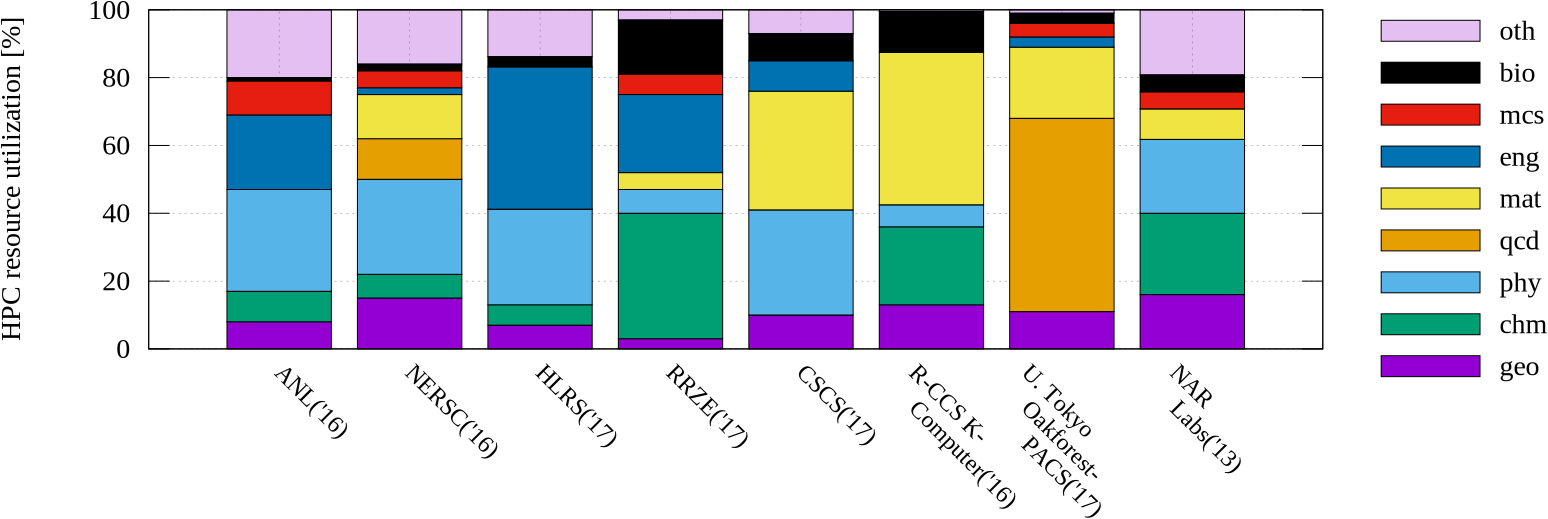
\includegraphics[width=\linewidth]{sys-util}
    \caption{\label{fid:disc:breakdown} Annual HPC site/system utilization by domain; Labels acc. to Table~\ref{table:APP}: \texttt{geo} = Geo-/Earthscience, \texttt{chm} = Chemistry, \texttt{phy} = Physics, \texttt{qcd} = Lattice QCD, \texttt{mat} = Material Science/Engineering, \texttt{eng} = Engineering (Mechanics, CFD), \texttt{mcs} = Math/Computer Science, \texttt{bio} = Bioscience, \texttt{oth} = \textit{Other}}
\end{figure}

\begin{comment}
\begin{table*}[tbp]
\begin{tabular}{|l|l|l|l|c|c|c|c|c|c|c|c|c|}
\hline
\multicolumn{1}{|c|}{System} & \multicolumn{1}{c|}{Host Institution}     & Description                      & \multicolumn{1}{c|}{Year} & \begin{tabular}[c]{@{}c@{}}Geoscience/\\ Earthscience\end{tabular} & Chemistry & Physics & Lattice QCD & Material Science/Engineering & \begin{tabular}[c]{@{}c@{}}Engineering\\ (Mechanics, CFD)\end{tabular} & Math/Computer Science & Bioscience & Other \\ \hline
ANL                          & Argonne National Lab, USA                 & All compute resources of ALCC    & 2016                      & 8                                                                  & 9         & 30      & 0           & 0                            & 22                                                                     & 10                    & 1          & 20    \\ \hline
NERSC                        & NERSC, Lawrence Berkeley Lab, USA         & All compute resources of NERSC   & 2016                      & 15                                                                 & 7         & 33      & 12          & 13                           & 2                                                                      & 5                     & 2          & 11    \\ \hline
HLRS                         & HPC Center Stuttgart, DEU                 & All compute resources of HLRS    & 2017                      & 7                                                                  & 6         & 31      & 0           & 0                            & 42                                                                     & 0                     & 3          & 11    \\ \hline
RRZE                         & Erlangen Regional Computing Center, DEU   & All compute resources of RRZE    & 2017                      & 3                                                                  & 37        & 7       & 0           & 5                            & 23                                                                     & 6                     & 16         & 3     \\ \hline
CSCS                         & Swiss National Supercomputing Centre, CHE & All compute resources of CSCS    & 2017                      & 10                                                                 & 0         & 31      & 0           & 35                           & 9                                                                      & 0                     & 8          & 7     \\ \hline
R-CCS                        & RIKEN CCS, Japan, JPN                     & K supercomputer                  & 2016                      & 13                                                                 & 23        & 6       & 0           & 45                           & 0                                                                      & 0                     & 12         & 1     \\ \hline
U. Tokyo                     & U. Tokyo IIC, JPN                         & Oakforest-PACS supercomputer     & 2017                      & 11                                                                 & 0         & 0       & 57          & 21                           & 3                                                                      & 4                     & 3          & 1     \\ \hline
NARLabs                      & National Center for HPC, TWN              & All compute resources of NARLabs & 2013                      & 16                                                                 & 24        & 22      & 0           & 9                            & 0                                                                      & 5                     & 5          & 19    \\ \hline
\end{tabular}
\end{table*}
\end{comment}

\subsection{Memory-bound Applications}
\todo{suggestions/options for memory-bound codes:}
% - memory bound: doesn't matter if fp64 is gone
% - Move away from paying a premium for FLOPs, mention NASA's example (https://ntrs.nasa.gov/archive/nasa/casi.ntrs.nasa.gov/20170000291.pdf)

\subsection{Compute-bound Applications}
\todo{suggestions/options for compute-bound codes:
 a) library
 b) mixed precision
 c) emulated by 2 fp32
 d) hope for cpu support for faster emulation
 e) accept the perf hit :-(
}

\subsection{More Diversity in FPUs\cJD{not less?}}
% - option: suggest to ditch fp32 and emulate fp32 ops in fp64 units
% - mixed precision can't work (requ. hand tuning in each app) -> not practical
% - compute bound codes -> what if no FP64 anymore in new chips -> what will they do?


% - themes: time-to-solution is most important metric
% - instructions doesn't matter too much because most are memory-bound
% - apps have different requirements
% - people need to dive deeper into their workloads
% - suggestion: decouple notion of hpc apps need high FP64 and which architecture to choose => see if NASA has papers on their design choices?!
% - breakdown of node-hours on science fields across many hpc centers


